\documentclass[letterpaper,10pt,oneside]{article}
\usepackage[utf8]{inputenc}
\usepackage{setspace}
\usepackage{hyperref}

\usepackage{graphicx}
\graphicspath{{images/}}
\usepackage[export]{adjustbox}
\usepackage{longtable}
\usepackage[left=1in, right=3in, bottom=1.25in, top=1.25in]{geometry}

\pagenumbering{gobble}

\begin{document}

%%%%%%%%%%%%%%%%% Header %%%%%%%%%%%%%%%%%

\noindent  \LARGE{\textbf{Stian Steinbakken}}
\smash{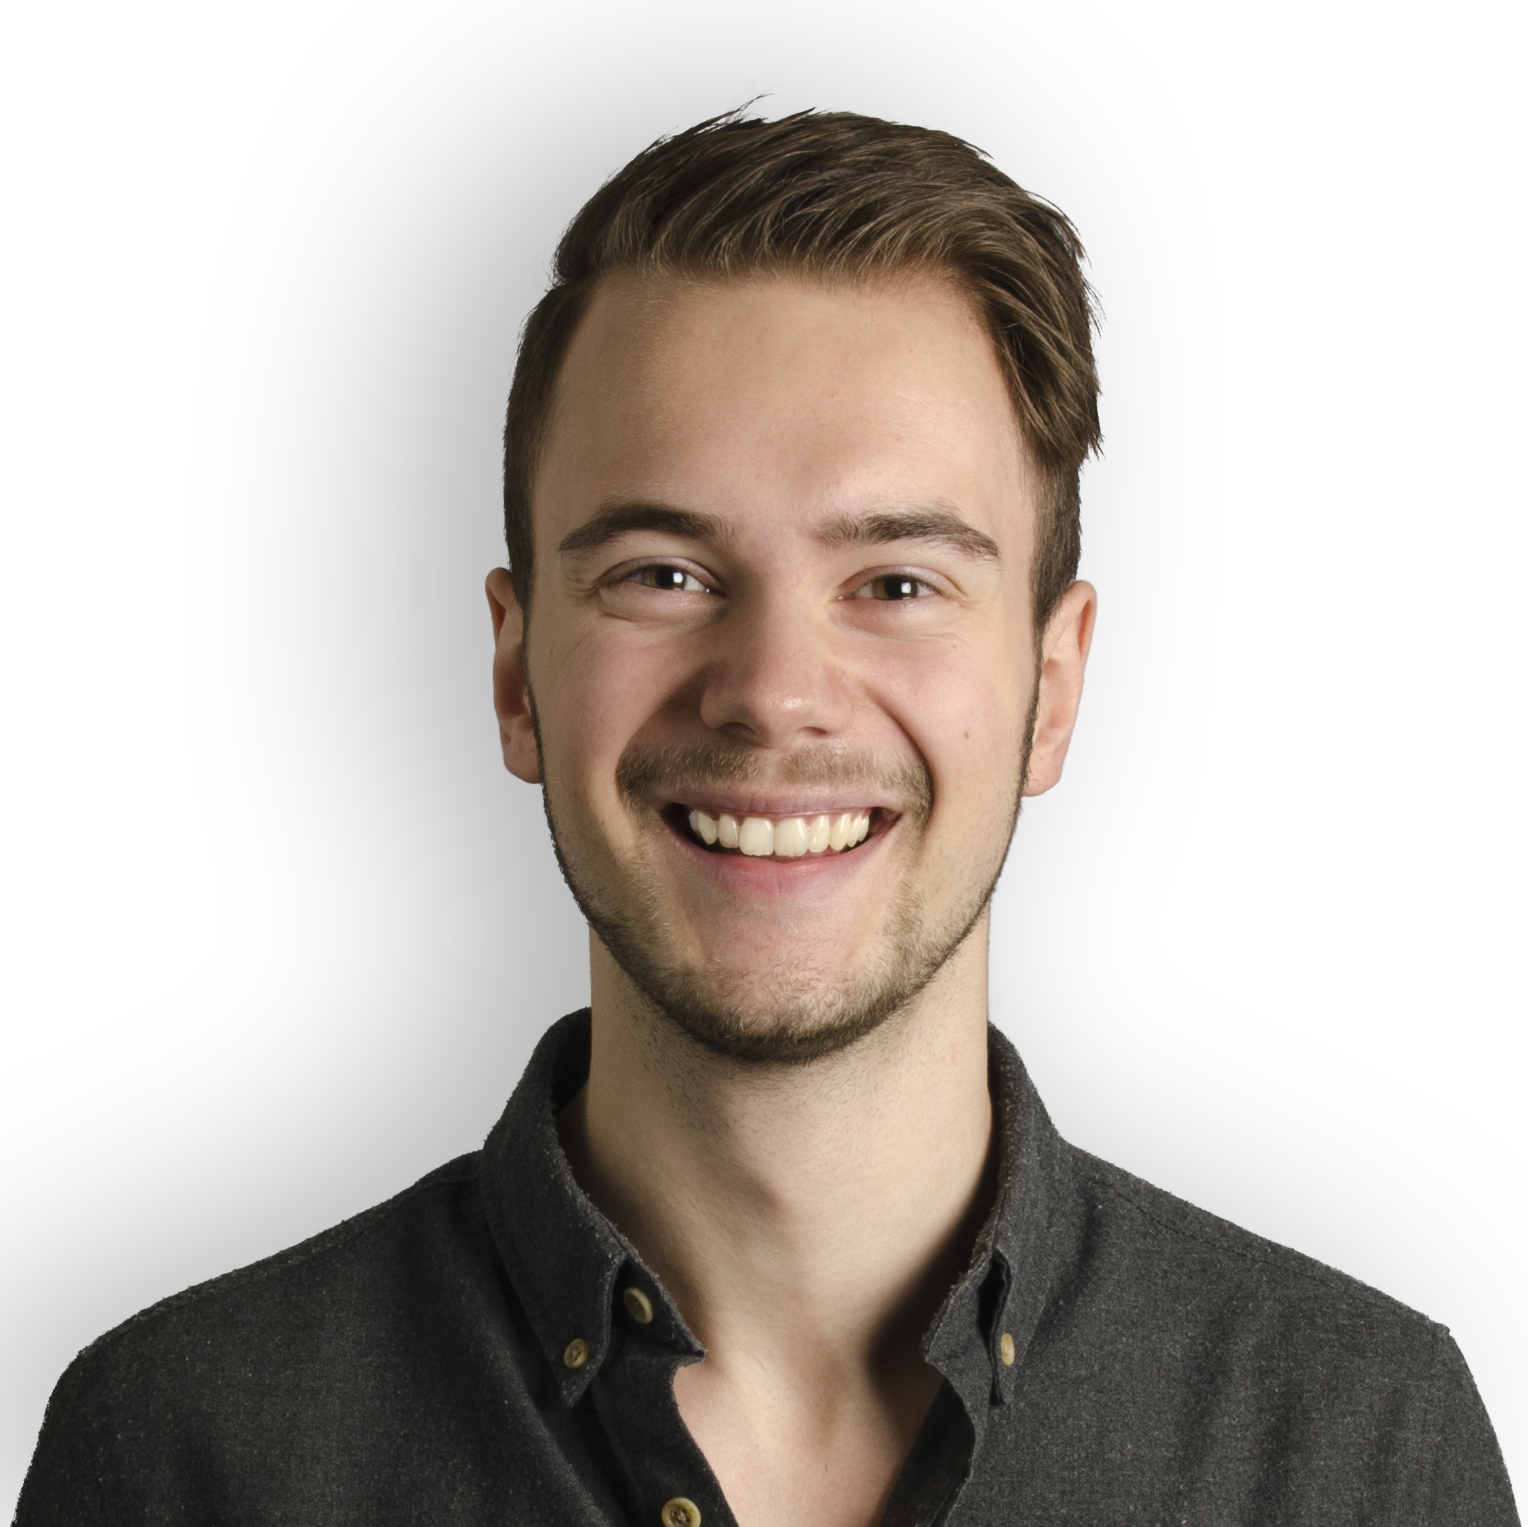
\includegraphics[scale=0.2, right]{CV}} \\
\vspace{-2ex}
\hline
\normalsize

%%%%%%%%%%%%%%%%% CONTACT INFORMATION %%%%%%%%%%%%%%%%%

\begin{center}
\begin{tabular}{l l}
\href{mailto:stiansteinbakken94@gmail.com}{stian@steinbakken.net}
 & \hspace{1in} LinkedIn: \href{https://www.linkedin.com/in/stianste/}{stianste}\\
 Wergelands vei 60, 8517 Narvik & \hspace{1in} GitHub: \href{https://github.com/stianste}{stianste}\Absender\\
 28. desember 1994 & \hspace{1in} Telefon: (+47) 97 423 430\\
\end{tabular}
\end{center}

\vspace{1em}

%%%%%%%%%%%%%%%%% MAIN BODY %%%%%%%%%%%%%%%%%%%%%%%%%%%

\noindent \begin{longtable}{@{} l l}
  \Large{Utdanning} & \textbf{NTNU – Norges teknisk-naturvitenskapelige universitet} \\
  & \textit{Sivilingeniør i Datateknologi, august 2014 - juni 2019}\\
     & Studieretning: kunstig intelligens.\\
     & \\
     \Large{Arbeidserfaring} 
     & \textbf{Junior Consulting AS} \\
     & \textit{Konsulent og prosjektleder, februar 2018 - d.d} \\
     & Jobber med forskjellige kundeprosjekter med utvikling og salg. Erfaring inkluderer \\
     & prosjektledelse på php prosjekt, og utvikler på prosjekt med React og Django.\\
     & \\
     & \textbf{Bekk Consulting AS} \\
     & \textit{Summer intern som utvikler, juli 2018 - august 2018} \\
     & Jobbet i et Scrum team på fire stykker med maskinlæring for Skatteetaten.\\
     & Teknologier inkluderer React-Redux, AWS Lambda, S3, DynamoDB og scikit-learn.\\
     & \\
     & \textbf{Capra Consulting AS} \\
     & \textit{Summer intern som utvikler, juni 2017 - august 2017} \\
     & Jobbet i et Scrum team på åtte hvor vi laget et CRM system for kunden Kinnetik.\\
     & Teknologier brukt inkluderer React-Redux, Webpack, AWS, Jenkins og Java Spring.\\
     & \\
     & \textbf{NTNU --- Norges teknisk-naturvitenskapelige universitet} \\
     & \textit{Studentassistent TDT4180 --- Menneske-maskin-interaksjon, januar 2017 - mai 2017}\\
     & Hjalp andre studenter i faget Menneske-maskin-interaksjon med Java programmering \\
     & og prinsipper i brukerinteraksjon.\\
     & \\
     & \textbf{NTNU --- Norges teknisk-naturvitenskapelige universitet} \\
     & \textit{Studentassistent TDT4113 --- Programmeringsprosjekt, august 2016 - desember 2016}\\
     & Hjalp andre studenter i faget Programmeringsprosjekt med design og programmering \\
     & av datasystemer som løser problemer i Python.\\
     & \\

 \Large{Frivillige verv}    & \textbf{Studentersamfundet i Trondhjem} \\
 & \textit{Webutvikler, august 2015 - d.d}\\
     & Toårig funksjonærverv hvor jeg primært jobber med videreutvikling av samfundet.no. \\
     & Teknologier brukt er Ruby, Ruby on Rails, SASS, haml, JavaScript, jQuery og React. \\
     & Lærer om å jobbe med et større system, Git og å jobbe i team.\\
     & \\
     & \textbf{Abakus --- linjeforeningen for Data- og kommunikasjonsteknologi} \\
     & \textit{Redaktør for linjeforeningsmagasinet «readme», mai 2016 - mai 2017}\\
     & Innebærte redaksjonelt ansvar for hele magasinet, samt å lede redaksjonen \\
     & bestående av nærmere 20 personer.
     & \\
     & \textbf{Abakus --- linjeforeningen for Data- og kommunikasjonsteknologi} \\
     & \textit{Styremedlem i Hovedstyret, mai 2016 - mai 2017}\\
     & \\
     & \textbf{Abakus --- linjeforeningen for Data- og kommunikasjonsteknologi} \\
     & \textit{Redaksjonsmedlem i «readme», september 2014 - d.d}\\
     & Skriver og gjør tidvis design på artikler. \\
     & Hadde også stilling som nestleder og økonomiansvarlig i ett år.\\
     & \\

\end{longtable}

Referanser oppgis ved forespørsel.

\end{document}

\iffalse{}
template: https://no.sharelatex.com/project/5986f770dcdfc926a22e7f86
\fi
